\documentclass[nobib, notoc, nolof, oneside, openany]{tufte-book}
% nobib     =   do not use package natbib, default in tufte-book.
%               it conflicts with biblatex.
% oneside   =   no blank page between chapters and page do not move
%               left or right based on the page number.
% symmetric = move left or right based on the page number
% openany   =

% ------------------------------------
% |            GEOMETRY              |
% ------------------------------------
\setcounter{tocdepth}{2}
\setcounter{secnumdepth}{2}

\makeatletter
% Paragraph indentation and separation for normal text
\renewcommand{\@tufte@reset@par}{
    \setlength{\RaggedRightParindent}{0pt}
    \setlength{\JustifyingParindent}{0pt}
    \setlength{\parindent}{0pt}
    \setlength{\parskip}{4pt}
}
\@tufte@reset@par

% Paragraph indentation and separation for marginal text
\renewcommand{\@tufte@margin@par}{
    \setlength{\RaggedRightParindent}{0pt}
    \setlength{\JustifyingParindent}{0pt}
    \setlength{\parindent}{0pt}
    \setlength{\parskip}{4pt}
}


\makeatletter
\renewcommand{\maketitlepage}{
    \begingroup
        \setlength{\parindent}{0pt}
            {\fontsize{24}{24}\selectfont\textit{\@author}\par}
        \vspace{1.75in}
            {\fontsize{36}{54}\selectfont\@title\par}
        \vspace{0.5in}
            {\fontsize{14}{14}\selectfont\textsf{\smallcaps{\@date}}\par}
        \vfill{\fontsize{14}{14}\selectfont\textit{\@publisher}\par}
        \thispagestyle{empty}
    \endgroup
}
\makeatother

\geometry{
    %showframe,             % DEBUG ONLY -- displays the margins
	left=13mm,              % left margin
	textwidth=135mm,        % width of main text
	marginparsep=8mm,       % gutter between main text block and margin notes
	marginparwidth=50mm     % width of margin notes
}
\fontsize{10}{20}\selectfont

% chapter format
\titleformat{\chapter}
    {\huge\rmfamily\itshape\color{red}}             % format applied to label+text
    {\llap{\colorbox{red}{\parbox{1.5cm}{\hfill\itshape\huge\color{white}\thechapter}}}}
    {2pt}   % horizontal separation between label and title body
    {}      % before the title body
    []      % after the title body

% section format
\titleformat{\section}
    {\normalfont\Large\itshape\color{orange}}       % format applied to label+text
    {\llap{\colorbox{orange}{\parbox{1.5cm}{\hfill\color{white}\thesection}}}}
    {1em}   % horizontal separation between label and title body
    {}      % before the title body
    []      % after the title body

% subsection format
\titleformat{\subsection}
    {\normalfont\large\itshape\color{blue}}% format applied to label+text
    {\llap{\colorbox{blue}{\parbox{1.5cm}{\hfill\color{white}\thesubsection}}}}
    {1em}   % horizontal separation between label and title body
    {}      % before the title body
    []      % after the title body

% ------------------------------------
% |        GENERIC PACKAGES          |
% ------------------------------------
% Math
\usepackage{amsmath,amsthm,amssymb,amsfonts}
\usepackage{stmaryrd}
\usepackage{relsize, xfrac}

% Pseudocode
\usepackage{clrscode3e}         % Pseudocode as in "Introduction to algorithms"
\usepackage{minted}             % Code highlighting

% Hyperlinks in PDFs
\usepackage{hyperref}

% Lorem Ipsum text
\usepackage{lipsum}

% Images
\usepackage{graphicx}
\setkeys{Gin}{width=\linewidth,totalheight=\textheight,keepaspectratio}
\graphicspath{/images}

% Verb environment
\usepackage{fancyvrb}           % Customization of verb environments.
\fvset{fontsize=\normalsize}    % Use a smaller font for the verb environment.

% Language
\usepackage[italian]{babel}

% Bibliography
\usepackage{csquotes}
\usepackage[
    backend=biber,
    style=alphabetic,
    sorting=ynt
]{biblatex}
\addbibresource{bib/bibliography.bib}

% Filter out some warning
\usepackage{silence}
  \WarningFilter*{latex}
    {Marginpar on page \thepage\space moved}
  \WarningFilter{biblatex}          % ONLY IF BIBLATEX DOES NOT USE IBID STYLE REF.
    {Patching footnote}

% IDK
\usepackage{booktabs}               % Makes prettier tables.
\usepackage{multicol}               % Small sections of multiple columns in
                                    % documents and tables.

\usepackage{bookmark}
\usepackage[
    activate={true,nocompatibility},
    final,
    tracking=true,
    nopatch=footnote,
    kerning=true,
    spacing=false,
    factor=1100,
    stretch=10,
    shrink=10
]{microtype}

\usepackage{pgf,tikz,tikz-cd}

\usepackage{fancyhdr}               % Custom headers and footers.
\pagestyle{fancyplain}              % Makes all pages in the document conform
                                    % to the custom headers and footers.
\fancyhead{}                        % No page header - if you want one, create
                                    % it in the same way as the footers below.
\fancyfoot[L]{}                     % Empty left footer.
\fancyfoot[C]{}                     % Empty center footer.
\fancyfoot[R]{\thepage}             % Page numbering for right footer.
\renewcommand{\headrulewidth}{0pt}  % Remove header underlines.
\renewcommand{\footrulewidth}{0pt}  % Remove footer underlines.
\setlength{\headheight}{13.6pt}     % Customize the height of the header.
\allowdisplaybreaks


% ------------------------------------
% |      THEOREM ENVIRONMENTS        |
% ------------------------------------
\newtheorem{thm}{Theorem}
\newtheorem{cor}[thm]{Corollary}
\newtheorem{prop}[thm]{Proposition}
\newtheorem{lem}[thm]{Lemma}
\newtheorem{conj}[thm]{Conjecture}
\newtheorem{quest}[thm]{Question}
\newtheorem{claim}{Claim}
\newtheorem{property}{Proprietà}

\theoremstyle{definition}
\newtheorem{defn}[thm]{Definition}
\newtheorem{defns}[thm]{Definitions}
\newtheorem{con}[thm]{Construction}
\newtheorem{exmp}[thm]{Example}
\newtheorem{exmps}[thm]{Examples}
\newtheorem{notn}[thm]{Notation}
\newtheorem{notns}[thm]{Notations}
\newtheorem{addm}[thm]{Addendum}
\newtheorem{exer}[thm]{Exercise}

\theoremstyle{remark}
\newtheorem{rem}[thm]{Osservazione}
\newtheorem{ans}[thm]{Answer}
\newtheorem{rems}[thm]{Remarks}
\newtheorem{warn}[thm]{Warning}
\newtheorem{sch}[thm]{Scholium}



% ------------------------------------
% |       COMMAND DEFINITIONS        |
% ------------------------------------
% Operators
\newcommand{\Mod}[1]{\ (\text{mod}\ #1)}
\newcommand{\N}{\mathbb{N}}
\newcommand{\Z}{\mathbb{Z}}
\newcommand{\Q}{\mathbb{Q}}
\newcommand{\R}{\mathbb{R}}
\newcommand{\C}{\mathbb{C}}
\newcommand{\OR}{\,|\,}
\newcommand{\AND}{\,\&\,}
\newcommand{\NOT}{!}

% Parenthesis
\newcommand{\bra}[1]{\left(#1\right)}
\newcommand{\sbra}[1]{\left[#1\right]}
\newcommand{\cbra}[1]{\left\{#1\right\}}
\newcommand{\norm}[1]{\left\lVert#1\right\rVert}
\newcommand{\ang}[1]{\left\langle#1\right\rangle}

% Shortened versions
\newcommand{\tn}[1]{\textnormal{#1}}

% Other
\DeclareMathOperator*{\argmin}{argmin}
\DeclareMathOperator*{\argmax}{argmax}
\newcommand{\upperAccE}{È \,}

% ------------------------------------
% |    DOCUMENT-SPECIFIC PACKAGES    |
% ------------------------------------

% Optimization problems
\usepackage{optidef}

% Derivation trees
\usepackage{bussproofs}

% ------------------------------------
% |    DOCUMENT-SPECIFIC COMMANDS    |
% ------------------------------------
% Utilities for Hoare logic
\newcommand{\Hoaretriple}[3]{
    \left\{\,#1\,\right\}
    \mathrel{#2}\nolinebreak
    \left\{\,#3\,\right\}
}

% Utilities for CCS
\newcommand{\strongTrans}[1]{\overset{#1}{\longrightarrow}}
\newcommand{\weakTrans}[1]{\overset{#1}{\Longrightarrow}}
\newcommand{\strongTrace}{\overset{\tn{T}}{\sim}}
\newcommand{\weakTrace}{\overset{\tn{T}}{\approx}}
\newcommand{\strongBisim}{\overset{\tn{BIS}}{\sim}}
\newcommand{\weakBisim}{\overset{\tn{BIS}}{\approx}}
\newcommand{\congr}{\overset{C}{\approx}}
\newcommand{\notCongr}{\overset{C}{\not\approx}}

% Utilities for Petri's nets
\newcommand{\event}{\mathrel{\fbox{$\phantom{\circ}$}}\,}
\newcommand{\fPlace}{
    \mathop{\tikz[baseline=-2.5]{\draw[thick](0,0)circle[radius=2.5mm];}}\,
}
\newcommand{\tPlace}{
    \mathop{
        \tikz[baseline=-2.5]{
            \draw[thick](0,0)circle[radius=2.5mm];
            \draw[fill] (0,0)circle[radius=1.3mm];
        }
    }\,
}
\newcommand{\preCond}[1]{{^\bullet}#1}
\newcommand{\postCond}[1]{#1^\bullet}
\newcommand{\canFire}[3]{#1\,[#2\rangle\,#3}

% Utilities for LTL
\newcommand{\nextOp}{\tn{\textbf{X}}}
\newcommand{\finallyOp}{\tn{\textbf{F}}}
\newcommand{\globallyOp}{\tn{\textbf{G}}}
\newcommand{\untilOp}{\tn{\textbf{U}}}
\newcommand{\weakOp}{\tn{\textbf{W}}}
\newcommand{\releaseOp}{\tn{\textbf{R}}}


% ------------------------------------
% |          MAIN SECTION            |
% ------------------------------------

\title{
    Modelli della\\
    Concorrenza
}
\author{Mattia Bolognini}
\date{Ultima modifica: \today}

\begin{document}

\maketitle

\tableofcontents

\chapter{Logica di Hoare}
\section{Definizione della logica}
La logica di Hoare è una logica utilizzata per dimostrare la correttezza di programmi sequenziali imperativi.

Si basa sul concetto di tripla:
\begin{center}
    $\Hoaretriple{\alpha}{C}{\beta}$
\end{center}
dove:
\begin{itemize}
    \item $\alpha$, detta precondizione, è una WFF della logica proposizionale che deve essere vera sullo stato della memoria prima di eseguire $C$;
    \item $C$, detto comando, è il codice che deve essere eseguito;
    \item $\beta$, detta post-condizione, è una WFF della logica proposizionale che deve essere vera sullo stato della memoria dopo l'esecuzione di $C$.
\end{itemize}
Di conseguenza una tripla di questo tipo viene letta come:
\begin{center}
    \textit{Se $\alpha$ è vera sullo stato della memoria prima di eseguire $C$ e $C$ termina, allora $\beta$ deve essere vero per lo stato della memoria dopo l'esecuzione di $C$.}
\end{center}
Se si dimostra questa affermazione, allora il programma \tn{C} è corretto.

Un linguaggio di programmazione, per essere NP-completo, deve poter:
\begin{itemize}
    \item assegnare un valore a una variabile;
    \item modificare il flusso di esecuzione del programma;
    \item poter iterare una o più isruzioni.
\end{itemize}
La logica di Hoare è NP-completa, perchè possiede un'istruzione di assegnamento, un'istruzione di scelta, e un'istruzione di iterazione. 

Per definire la struttura valida di un programma nella logica di Hoare, è necessario prima definire l'insieme $E$ delle espressioni aritmetiche e l'insieme $B$ delle formule booleane.\\
Grammatica delle espressioni aritmetiche:
\begin{itemize}
    \item $\forall v \in V$ (insieme delle variabili), $v \in E$;
    \item $\forall z \in \mathbb{Z}$, $z \in E$;
    \item $\forall e_1, e_2 \in E$, $(e_1+e_2), (e_1-e_2), (e_1*e_2), (e_1/e_2) \in E$.
\end{itemize}
Grammatica delle espressioni booleane:
\begin{itemize}
    \item $\textnormal{true}, \textnormal{false} \in B$;
    \item $\forall b_1, b_2 \in B$, $(b_1 \AND b_2), (b_1 \OR b_2), \NOT b_1 \in B$;
    \item $\forall e_1, e_2 \in E$, $(e_1 < e_2), (e_1 = e_2), (e_1 != e_2), (e_1 \le e_2) \in B$.
\end{itemize}

Sia $C$ l'insieme dei programmi (detti comandi) validi della logica di Hoare, allora la grammatica per $C$ è:
\begin{itemize}
    \item istruzione di skip $\in C$:
    \begin{center}
        skip
    \end{center}
    \item istruzione di assegnamento $\in C$:
    \begin{center}
        $v:=e \quad v \in V \land e \in E$
    \end{center}
    \item istruzione di scelta $\in C$:
    \begin{center}
        if $b$ then $c_1$ else $c_2$ endif $\quad b \in B \land c_1, c_2 \in C$
    \end{center}
    \item istruzione di iterazione $\in C$:
    \begin{center}
        while $b$ do $c$ endwhile $\quad b \in B \land c \in C$
    \end{center}
    \item istruzione di sequenza $\in C$:
    \begin{center}
        $c_1 ; c_2 \quad c_1, c_2 \in C$
    \end{center}
\end{itemize}

L'apparato deduttivo contiene tutte le regole di inferenza, che permettono di derivare nuove triple valide a partire da triple già presenti.
Viene utilizzato per dimostrare la correttezza di un programma. Tutte le regole di inferenza sono corrette, ovvero se le triple premesse sono dimostrate e si può derivare da esse una nuova tripla tramite una regola, allora la tripla derivata è dimostrata.

\begin{itemize}
    \item regola della sequenza:
    \begin{center}
        \begin{prooftree}
            \AxiomC{$\Hoaretriple{p_1}{C}{p_2}$}
            \AxiomC{$\Hoaretriple{p_2}{D}{p_3}$}
            \BinaryInfC{$\Hoaretriple{p_1}{C;D}{p_3}$}
        \end{prooftree}
    \end{center}
    \item regola della scelta:
    \begin{center}
        \begin{prooftree}
            \AxiomC{$\Hoaretriple{p \land b}{C}{q}$}
            \AxiomC{$\Hoaretriple{p \land \tn{¬b}}{D}{q}$}
            \BinaryInfC{$\Hoaretriple{p}{\tn{if } b \tn{ then } C \tn{ else } D \tn{ endif}}{q}$}
        \end{prooftree}
    \end{center}
    \item regola di skip:
    \begin{center}
        \begin{prooftree}
            \AxiomC{}
            \UnaryInfC{$\Hoaretriple{p}{\tn{skip}}{p}$}
        \end{prooftree}
    \end{center}
    \item regola dell'implicazione (su pre-condizione):
    \begin{center}
        \begin{prooftree}
            \AxiomC{$p' \rightarrow p$}
            \AxiomC{$\Hoaretriple{p}{C}{q}$}
            \BinaryInfC{$\Hoaretriple{p'}{C}{q}$}
        \end{prooftree}
    \end{center}
    \item regola dell'implicazione (su post-condizione):
    \begin{center}
        \begin{prooftree}
            \AxiomC{$\Hoaretriple{p}{C}{q}$}
            \AxiomC{$q \rightarrow q'$}
            \BinaryInfC{$\Hoaretriple{p}{C}{q'}$}
        \end{prooftree}
    \end{center}
    \item regola dell'assegnamento:
    \begin{center}
        \begin{prooftree}
            \AxiomC{}
            \UnaryInfC{$\Hoaretriple{q[\sfrac{E}{x}]}{x:=E}{q}$}
        \end{prooftree}
    \end{center}
    dove $\cbra{q}$ è un WFF che può contenere la variabile $x$, mentre $\cbra{q[\sfrac{E}{x}]}$ è l'espressione $q$ in cui però ogni occorrenza di $x$ è stata sostituita con l'espressione $E$.

    La logica ammette anche casi in cui l'espressione $E$ contenga a sua volta la stessa variabile su cui si sta procedendo con l'assegnamento, in questo caso $x$  
    \footnote{
        Esempio di derivazione della pre-condizione in cui l'espressione contiene a sua volta la variabile:\\
        $\Hoaretriple{q[\sfrac{i+1}{i}]}{i = i + 1}{s=x^i}$\\
        $\cbra{q[\sfrac{i+1}{i}]} = \cbra{s=x^{i+1}}$\\
        $\Hoaretriple{s=x^{i+1}}{i = i + 1}{s=x^i}$
    }.
    
    \item regola di iterazione (per sola correttezza parziale):
    \begin{center}
        \begin{prooftree}
            \AxiomC{$\Hoaretriple{\alpha \land \beta}{C}{\alpha \land \tn{def}(E)}$}
            \UnaryInfC{$\Hoaretriple{\alpha \land \tn{def}(E)}
                                    {\tn{while } \beta \tn{ do } C \tn{ endwhile}}
                                    {\alpha \land \tn{¬}B}$}
        \end{prooftree}
    \end{center}
    $\alpha$ è una WFF vera prima dell'esecuzione di $W$ e a seguito di qualsiasi iterazione, e prende il nome di \textbf{invariante di ciclo}.
\end{itemize}

\section{Dimostrazione di correttezza}
Dimostrare la correttezza di un programma (imperativo) usando la logica di Hoare significa dimostrare semplicemente la validità di una tripla $\Hoaretriple{p}{C}{q}$ usando l'apparato deduttivo della logica, dove $C$ è il programma da dimostrare, $\cbra{q}$ è la WFF che esprime ciò che il programma dovrebbe fare (il risultato atteso in funzione degli input), mentre $\cbra{p}$ è la WFF che esprime dei vincoli sui valori di input che si assumono veri prima dell'esecuzione del programma. La dimostrazione della correttezza di una tripla si divide in:
\begin{itemize}
    \item dimostrazione di \textbf{correttezza parziale}: viene dimostrata la derivabilità della tripla
    \footnote{La derivabilità implica la correttezza della tripla, in quanto la logica di Hoare è una logica corretta. La logica di Hoare non è però completa, in quanto più potente dell'aritmetica di Peano (vedi i teoremi di Godel).}.
    \item dimostrazione di \textbf{correttezza totale}: viene dimostrata sia la derivabilità della tripla che la terminazione di eventuali istruzioni di iterazione.
\end{itemize}
\begin{defn}
    Una \textbf{variante} di ciclo è un'espressione aritmetica $E$ tale per cui:
    \begin{itemize}
        \item $\tn{inv} \rightarrow E \ge 0$
        \item $\Hoaretriple{\tn{inv} \land \beta \land E = k \land E > 0}{C}{\tn{inv} \land E < k}$ \footnote{$k$ è una variabile di appoggio utilizzata per memorizzare il valore di $E$ prima dell'esecuzione di $C$, in modo da poterlo confrontare con il nuovo valore di $E$ al termine dell'esecuzione di $C$.} è una tripla derivabile, e quindi il valore assunto da $E$ diminuisca a seguito di ogni esecuzione di $C$.
    \end{itemize}
\end{defn}
Riuscire a trovare una variante per un'istruzione di iterazione implica la correttezza totale dell'istruzione di iterazione.

\begin{exmp}
    Dimostrare la correttezza della tripla:
    \begin{center}
        $\Hoaretriple{x>1}{y:=x+1}{y>1}$
    \end{center}
    A partire da $y:=x+1 \cbra{y>1}$, cerco di derivare una precondizione $p'$ tale per cui $x>1 \rightarrow p'$.
    Per la regola dell'assegnamento:
    \begin{center}
        $\vDash \Hoaretriple{x+1>1}{y:=x+1}{y>1}$
    \end{center}
    che si può riscrivere come:
    \begin{center}
        $\vDash \Hoaretriple{x>0}{y:=x+1}{y>1}$
    \end{center}
    Per la regola dell'implicazione (sulla pre-condizione):
    \begin{center}
        \begin{prooftree}
            \AxiomC{$x>1 \rightarrow x>0$}
            \AxiomC{$\Hoaretriple{x>0}{y:=x+1}{y>1}$}
            \BinaryInfC{$\Hoaretriple{x>1}{y:=x+1}{y>1}$}
        \end{prooftree}
    \end{center}
    Sono quindi riuscito a derivare la tripla che si voleva dimostrare.
    La tripla di partenza è quindi dimostrata.
\end{exmp}

\begin{exmp}
    Dimostrare la correttezza della tripla:
    \begin{center}
        $\Hoaretriple{s=x^i \land i < N}{i:=i+1; s:=s*x}{s=x^i \land i \le N}$
    \end{center}
    Il comando è composto da due istruzioni di assegnamento, e sarebbe quindi necessario applicare due volte la regola di assegnamento.
    Quando gli assegnamenti consecutivi sono indipendenti \footnote{Per assegnamenti indipendenti si intende che se è presente un assegnamento a una certa variabile, allora quella variabile non può comparire nelle espressioni aritmetiche degli altri assegnamenti.}, però, è possibile effettuare contemporaneamente tutte le sostituzioni sulla post-condizione.
    \begin{center}
        $\vDash \Hoaretriple{s*x=x^{i+1} \land i+1 \le N}{i:=i+1; s:=s*x}{s=x^i \land i \le N}$
    \end{center}
    che si può riscrivere come:
    \begin{center}
        $\vDash \Hoaretriple{s=x^i \land i+1 \le N}{i:=i+1; s:=s*x}{s=x^i \land i \le N}$
    \end{center}
    Per la regola dell'implicazione (sulla pre-condizione):
    \begin{prooftree}
        \AxiomC{ $i < N \rightarrow i+1 \le N$ }
        \AxiomC{ $\Hoaretriple{\begin{aligned}
            &s*x=x^{i+1}\\
            &\land \; i+1 \le N
        \end{aligned}}
        {\begin{aligned}
            &i:=i+1;\\
            &s:=s*x
        \end{aligned}}
        {\begin{aligned}
            &s=x^i\\
            &\land i \le N
        \end{aligned}}$ }
        \BinaryInfC{ $\Hoaretriple{s=x^i \land \; i < N}
        {\begin{aligned}
            &i:=i+1; \\
            &s:=s*x
        \end{aligned}}
        {s=x^i \land \; i \le N}$ }
    \end{prooftree}
    Si è quindi riusciti a derivare la tripla di partenza. La tripla di partenza è quindi dimostrata.
\end{exmp}

\begin{exmp}
    Dimostrare la correttezza della tripla:
    \begin{center}
        $\Hoaretriple{\textnormal{T}}
        {\begin{aligned}
            & \textnormal{if } x<y\\
            & \textnormal{then } m:=y\\
            & \textnormal{else } m:=x\\
            & \textnormal{endif}
        \end{aligned}}
        {m \ge x \land m \ge y \land (m=x \lor m=y)}$
    \end{center}
    Usando la regola di scelta al contrario, la tripla può essere scomposta in due triple:
    \begin{center}
        $t_1 = \Hoaretriple{x<y}{m:=y}{m \ge x \land m \ge y \land (m=x \lor m=y)}$\\
        $t_2 = \Hoaretriple{x \ge y}{m:=x}{m \ge x \land m \ge y \land (m=x \lor m=y)}$
    \end{center}
    Bisogna quindi dimostrare la correttezza di entrambe le triple.
    Considerando $t_1$, per la regola dell'assegnamento:
    \begin{center}
        $\vDash \Hoaretriple{\begin{aligned}
            &y \ge x \land y \ge y\\
            &\land (y = x \lor y = y)
        \end{aligned}}
        {m:=y}
        {\begin{aligned}
            &m \ge x \land m \ge y\\
            &\land (m=x \lor m=y)
        \end{aligned}}$
    \end{center}
    che si può riscrivere come:
    \begin{center}
        $\vDash \Hoaretriple{y \ge x}{m:=y}
        {\begin{aligned}
            &m \ge x \land m \ge y\\
            &\land (m=x \lor m=y)
        \end{aligned}}$
    \end{center}
    Per la regola dell'implicazione (sulla pre-condizione):
    \begin{prooftree}
        \AxiomC{$x<y \rightarrow y \ge x$}
        \AxiomC{$\Hoaretriple{y \ge x}{m:=y}
        {\begin{aligned}
            &m \ge x \land m \ge y\\
            &\land (m=x \lor m=y)
        \end{aligned}}$}
        \BinaryInfC{$\Hoaretriple{x<y}{m:=y}
        {m \ge x \land m \ge y \land (m=x \lor m=y)}$}
    \end{prooftree}
    Si è quindi riusciti a derivare $t_1$, e quindi si è dimostrata la sua correttezza.\\
    Considerando $t_2$, per la regola dell'assegnamento:
    \begin{center}
        $\vDash \Hoaretriple{\begin{aligned}
            &x \ge x \land x \ge y\\ 
            &\land (x=x \lor x=y)
        \end{aligned}}
        {m:=x}
        {\begin{aligned}
            &m \ge x \land m \ge y\\
            &\land (m=x \lor m=y)
        \end{aligned}}$
    \end{center}
    che si può riscrivere come:
    \begin{center}
        $\vDash \Hoaretriple{x \ge y}{m:=x}{\begin{aligned}
            &m \ge x \land m \ge y\\
            &\land (m=x \lor m=y)
        \end{aligned}}$
    \end{center}
    Si è quindi riusciti a derivare $t_2$, e quindi si è dimostrata la sua correttezza.\\
    Avendo dimostrato la correttezza di entrambe le triple, allora anche la tripla di partenza è dimostrata.
\end{exmp}

Per dimostrare la correttezza di una tripla della forma $\{ p \} x:=E \{ q \}$ si deve partire considerando solo comando e la post-condizione. Usando la regola dell'assegnamento, si deriva la pre-condizione $q[\sfrac{E}{x}]$.
    Se $q[\sfrac{E}{x}] \rightarrow p$ (implicazione logica), allora la tripla di partenza è dimostrata.

    
\chapter{Calculus of Communicating Systems}
Il Calculus of Communicating System (CCS) è un linguaggio per descrivere i processi di sistemi anche concorrenti, e offre un modo di eseguire operazioni sui processi.

Il linguaggio dei processi CCS, ovvero espressioni CCS che descrivono processi validi, è definito dalla seguente grammatica:
\begin{itemize}
    \item 
\end{itemize}
\chapter{Reti di Petri}
\section{Introduzione}
Le reti di Petri sono un modello formale per la descrizione di sistemi
distribuiti a tempo discreto. A differenza delle algebre di processo, come il CCS,
le reti di Petri permettono di descrivere la true concurrency di un
sistema concorrente, usando una semantica a ordine parziale.
A differenza del CCS, che analizza lo stato globale del sistema concorrente,
le reti di Petri permettono di rappresentare l'evoluzione degli stati
delle singole parti che compongono il sistema, senza dover esplicitamente
trattare lo stato globale del sistema concorrente (che molto spesso è
sconosciuto).\\
Le reti di Petri sono utili per verificare le proprietà di un sistema concorrente,
come liveness e assenza di deadlock, in modo da dimostrarne la correttezza.
Alcuni problemi di decisione su reti di Petri sono stati studiati da
Esparza e Nielsen (1995) METTERE CITAZIONE.

\section{Reti, eventi e grafi dei casi}
Le reti di Petri sono sistemi a transizione di stati che estendono la
classe delle reti elementari.
\begin{defn}
    Una \textbf{rete} è
\end{defn}

\begin{defn}
    Una \textbf{rete elementare} è
\end{defn}

\begin{defn}
    Una \textbf{rete di Petri} è una quadrupla $N = (P, T, F, m_0, W)$ tale che:
    \begin{itemize}
        \item $P$ è un insieme finito di \textbf{posti}
        \footnote{Con posto si intende lo stato di una parte del sistema
        che si vuole rappresentare. Lo stato globale farà invece riferimento a
        tutto il sistema.}.\\
        Un posto può essere visto come una condizione sul sistema che
        si vuole rappresentare.
        \item $T$ è un insieme finito di \textbf{transizioni}, dette anche
        eventi.
        \item $F \subseteq (B\times E)\cup(E\times B)$
        è una \textbf{relazione di flusso}, ovvero un insieme di
        archi diretti che collegano i posti alle transizioni e le transizioni
        ai posti. Gli archi non possono essere definiti tra posti e tra
        transizioni
        \footnote{Si può osservare che una rete definisce un grafo bipartito,
        dove i due sottoinsiemi che definiscono la partizione sono $P$ ed $T$.}.
        Per definizione, inoltre, ogni evento della rete ha almeno uno stato
        locale di ingresso e almeno uno stato locale di uscita.
        \[
            \forall e \in E, \exists p, q \in B : (p, e) \in F \land
            (e, q) \in F.
        \]
        \item $m_0$ è la marcatura iniziale della rete, che specifica quanti
        token sono presenti in ogni posto della rete di Petri.
        \item $W: F \rightarrow \mathbb{Z}$ è una funzione che assegna a ogni
        arco della rete un peso, rappresentante la sua molteplicità.
    \end{itemize}
\end{defn}
Senza perdere di generalità, si possono considerare le sole reti di Petri
in cui la funzione $W$ assegna a ogni arco della rete un peso pari a 1,
e in cui ogni posto ha una capacità di token massima pari a 1.
In questo caso, inoltre, la marcatura della rete di Petri collassa a una semplice
configurazione, ovvero a un sottoinsieme di posti della rete.
D'ora in poi verranno trattate solo reti di Petri di questo tipo, in modo
da semplificarne la trattazione.

Graficamente, gli elementi di una rete di Petri sono rappresentati come:
\begin{itemize}
    \item stato locale falso: $\fPlace$
    \item stato locale vero: $\tPlace$
    \item evento: $\event$
    \item transizione: $\longrightarrow$
\end{itemize}

\begin{defn}
    Dato un elemento $x \in B \cup E$, è possibile definire i due seguenti
    insiemi:
    \begin{align*}
        \preCond{x} &= \cbra{y \in B \cup E : (y, x) \in F}\\
        \postCond{x} &= \cbra{y \in B \cup E : (x, y) \in F}
    \end{align*}
    Se $x$ è un evento, allora $\preCond{x}$ sono le \textbf{pre-condizioni} di
    $x$, mentre $\postCond{x}$ sono le \textbf{post-condizioni} di $x$.\\
    Se invece $x$ è uno stato locale, $\preCond{x}$ sono i \textbf{pre-eventi}
    di $x$, mentre $\postCond{x}$ sono i \textbf{post-eventi} di $x$.

    \upperAccE possibile estendere la definizione di questi due insiemi anche
    a insiemi di stati locali ed eventi. Sia $X \subseteq B \cup E$, allora:
    \begin{align*}
        \preCond{X} &= \bigcup\limits_{x \in X} \preCond{x}\\
        \postCond{X} &= \bigcup\limits_{x \in X} \postCond{x}
    \end{align*}
\end{defn}

\begin{defn}
    Una rete di Petri è \textbf{semplice} sse:
    \[
        \forall x, y \in B \cup E, \preCond{x} = \preCond{y} \land
        \postCond{x} = \postCond{y} \rightarrow x = y
    \]
    \begin{marginfigure}[-5cm]
        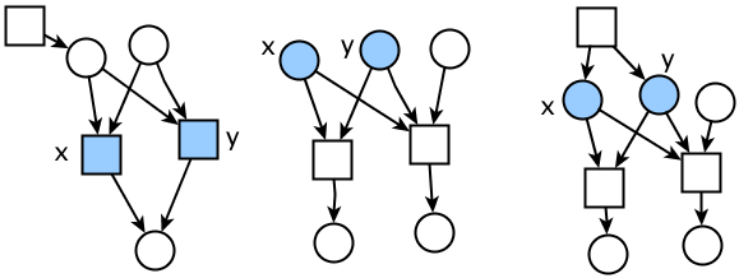
\includegraphics[width=1\linewidth]{img/reti_non_semplici.png}
        \caption{Reti non semplici}
        \label{fig:reti_non_semplici}
    \end{marginfigure}
\end{defn}

\begin{defn}
    Una rete di Petri è \textbf{pura} sse:
    \[
        \forall e \in E, \preCond{e} \cap \postCond{e} = \emptyset
    \]
    \begin{marginfigure}[-1cm]
        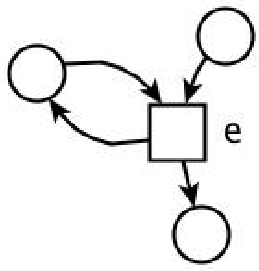
\includegraphics[width=0.4\linewidth]{img/rete_non_pura.png}
        \caption{Rete non pura.}
        \label{fig:rete_non_pura}
    \end{marginfigure}
\end{defn}

\begin{defn}
    Un evento $e$ è \textbf{abilitato} in una rete $N$ per la configurazione
    corrente $c$ sse:
    \[
        \preCond{e} \subseteq c \land \postCond{e} \cap c = \emptyset
    \]
    ovvero tutte le sue pre-condizioni sono vere, mentre tutte le sue
    post-condizioni sono false.\\
    La configurazione del sistema dopo aver eseguito $e$, indicata con $c'$,
    sarà:
    \[
        c' = \bra{c \setminus \preCond{e}} \cup \postCond{e}
    \]
    L'occorrenza di un evento $e$ nella configurazione corrente $c$ che porta
    alla configurazione $c'$ viene indicata con $\canFire{c}{e}{c'}$.
\end{defn}

\begin{defn}
    Un insieme di eventi $U \subseteq T$ è un \textbf{passo} sse tutti i suoi
    eventi sono indipendenti, ovvero eventi diversi di $U$ non condividono
    alcuno stato locale.
    \[
        \forall e_1, e_2 \in U, e_1 \neq e_2 \rightarrow
        (\preCond{e_1} \cup \postCond{e_1}) \cap
        (\preCond{e_2} \cup \postCond{e_2}) = \emptyset
    \]
\end{defn}

\begin{defn}
    Un insieme di eventi $U \subseteq T$ è un \textbf{passo abilitato}
    per la configurazione corrente $c$ sse:
    \[
        U \tn{ è un passo } \land \forall e \in U, \canFire{c}{e}{}
    \]
\end{defn}

\begin{defn}
    Siano $N_1 = (B_1, E_1, F_1)$ e $N_2 = (B_2, E_2, F_2)$ due sistemi
    elementari, $N_2$ è \textbf{sottorete} di $N_1$ sse:
    \begin{itemize}
        \item $B_2 \subseteq B_1$
        \item $E_2 \subseteq E_1$
        \item $F_2 = F_1 \cap \bra{\bra{B_2 \times E_2} \cup \bra{E_2 \times B_2}}$
    \end{itemize}
\end{defn}

\begin{defn}
    Sia $N = (B, E, F)$ una rete, la \textbf{sottorete generata da
    un sottoinsieme di stati locali} $B_1 \subseteq B$ è la rete
    $N_1 = (B_1, E_1, F_1)$ con:
    \begin{itemize}
        \item $E_1 = \preCond{B_1} \cup \postCond{B_1}$
        \item $F_1 = F \cap\bra{\bra{B_1 \times E_1} \cup \bra{E_1 \times B_1}}$
    \end{itemize}
\end{defn}

\begin{defn}
    Sia $N = (B, E, F)$ una rete, la \textbf{sottorete generata da un
    sottoinsieme di eventi} $E_1 \subseteq E$ è la rete
    $N_1 = (B_1, E_1, F_1)$ con:
    \begin{itemize}
        \item $B_1 = \preCond{E_1} \cup \postCond{E_1}$
        \item
        $F_1 = F \cap \bra{\bra{B_1 \times E_1} \cup \bra{E_1 \times B_1}}$
    \end{itemize}
\end{defn}

\subsection*{Grafo dei casi e grafo dei casi sequenziale}
\begin{defn}
    L'\textbf{insieme delle configurazioni raggiungibili}
    $C_{\Sigma} \subseteq 2^{B}$ nella rete di Petri $(P, T, F, c_{\tn{start}})$
    è definito come:
    \begin{itemize}
        \item $c_{\tn{start}} \in C_{\Sigma}$
        \item $\bra{c \in C_{\Sigma} \land \exists U \subseteq T :
        \canFire{c}{U}{c'}} \rightarrow c' \in C_{\Sigma}$
    \end{itemize}
\end{defn}

\begin{defn}
    L'\textbf{insieme dei passi} $U_{\Sigma}$ di un sistema elementare $\Sigma$
    sono tutti i passi possibili che il sistema $\Sigma$ può compiere.
    \[
        U_{\Sigma} = \cbra{U \subseteq E \, | \,
        \exists c_1, c_2 \in C_{\Sigma} : \canFire{c_1}{U}{c_2}}
    \]
\end{defn}

Il comportamento di una rete di Petri
può essere descritto completamente con un grafo dei casi, in cui ogni nodo
rappresenta una delle possibili configurazioni raggiungibili della rete
e ogni arco $(c_i, c_j)$ etichettato con $U$ rappresenta l'esecuzione
$\canFire{c_i}{U}{c_j}$ di un passo abilitato $U$ per $c_i$.
Essendo un arco etichettato con un passo abilitato del sistema, il grafo
dei casi $CG_{\Sigma}$ descrive la \textbf{step semantics} del sistema
considerato.

\begin{defn}
    Il \textbf{grafo dei casi} $CG_{\Sigma}$ di una rete di Petri $\Sigma$ è
    formalmente definito come la quadrupla
    $(C_{\Sigma}, U_{\Sigma}, A, c_{\tn{start}})$ dove:
    \begin{itemize}
        \item $C_{\Sigma}$, l'insieme dei casi raggiungibili, è l'insieme
        dei nodi.
        \item $U_{\Sigma}$, l'insieme dei passi, è l'alfabeto del grafo.
        \item $A = \cbra{(c, U, c') \, | \, c, c' \in C_{\Sigma} \land
        U \in U_{\Sigma} \land \canFire{c}{U}{c'}}$
        è l'insieme degli archi
        \footnote{Ogni arco è quindi etichettato con un \textit{passo},
        ovvero con un insieme di eventi del sistema $\Sigma$.}.
        \item $c_{\tn{start}}$ è la configurazione di partenza.
    \end{itemize}
\end{defn}

\begin{property}
    Il grafo dei casi gode della \textbf{diamond property}.\\
    Se un grafo dei casi $CG_{\Sigma}$ per un sistema elementare
    $\Sigma = (C_{\Sigma}, U_{\Sigma}, A, c_{\tn{start}})$ presenta gli archi
    $(c_1, U_1, c_2)$, $(c_2, U_2, c_3)$ e $(c_1, U_2, c_4)$, con
    $c_1, c_2, c_3, c_4 \in C_{\Sigma} \land U_1, U_2 \in U_{\Sigma} \land
    U_1 \cap U_2 = \emptyset$,\\
    allora sicuramente il sistema $\Sigma$ ammetterà i passi
    $(c_4, U_1, c_3)$ e $(c_1, U_1 \cup U_2, c_3)$.
    \begin{marginfigure}[1cm]
        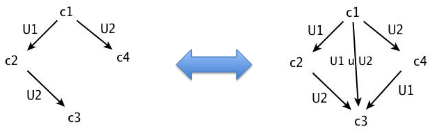
\includegraphics[width=1.05\linewidth]{img/diamond_property.png}
        \caption{Diamond property.}
        \label{fig:diamond_property}
    \end{marginfigure}
\end{property}
Gli archi del grafo dei casi sono etichettati
con un \textit{sottoinsieme} di eventi concorrenti che possono scattare dalla
configurazione di partenza. Questa semantica, come già detto, prende il nome di
step semantic.
Se però si è interessati a descrivere il comportamento del sistema concorrente
preso in analisi analizzando le possibili sequenze di eventi
che sono possibili al suo interno, senza interessarsi a quali eventi
possono essere eseguiti in maniera concorrente, allora è possibile definire
un grafo dei casi sequenziale. Il grafo dei casi sequenziale si differenzia
dal grafo dei casi solo per il fatto che i suoi archi sono etichettati con un
\textit{singolo evento}, senza quindi esplicitare un insieme di eventi
eseguibili concorrentemente.
La semantica descritta dal grafo dei casi sequenziale prende il nome
di semantica a \textbf{interleaving}, e altro non è
che una simulazione sequenziale non deterministica del sistema.

Il grafo dei casi sequenziale, inoltre, è, di fatto, un sistema a transizioni
etichettato che modella il sistema concorrente preso in analisi,
e può quindi essere usato per verificare alcune proprietà del sistema
concorrente che si sta analizzando.
Data una rete di Petri, però, trovare l'insieme delle configurazioni raggiungibili
può essere complesso e portare a un'esplosione combinatoria:
per verificare proprietà su un sistema concorrente, quindi, spesso
si preferisce ridursi a sottocasi di reti di Petri più facili da gestire,
o si preferiscono altri metodi formali, come le logiche temporali.

\begin{defn}
    Il \textbf{grafo dei casi sequenziale} $SCG_{\Sigma}$ di una rete
    di Petri $\Sigma$ è una quadrapla $(C_{\Sigma}, E, A, c_{\tn{start}})$
    dove:
    \begin{itemize}
        \item $C_{\Sigma}$, l'insieme dei casi raggiungibili, è l'insieme dei
        nodi.
        \item $E$, l'insieme degli eventi, è l'alfabeto del grafo con cui
        verranno etichettati gli archi.
        \item $A = \cbra{(c, e, c') \, | \, c, c' \in C_{\Sigma} \land
        e \in E \land \canFire{c}{e}{c'}}$
        è l'insieme degli archi.
        \item $c_{\tn{start}}$ è la configurazione di partenza.
    \end{itemize}
\end{defn}

\begin{marginfigure}
    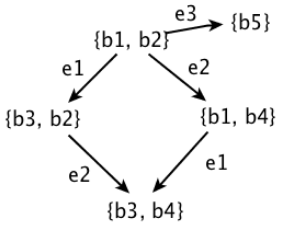
\includegraphics[width=0.60\linewidth]{img/grafo_casi_sequenziale.png}
    \caption{Grafo dei casi sequenziale.}
    \label{fig:sequential_case_graph}
\end{marginfigure}

\begin{property}
    Il grafo dei casi $CG_{\Sigma}$ e il grafo dei casi sequenziale
    $SCG_{\Sigma}$ della stessa rete di Petri $\Sigma$ sono
    \textbf{sintatticamente equivalenti}, ovvero è possibile ottenere uno a
    partire dall'altro usando solo procedimenti di modifica sintattica.
\end{property}

\begin{rem}
    Il grafo dei casi è un sistema di transizioni etichettato per il sistema
    concorrente descritto dalla rete.
    Trovare quindi un sistema di transizioni etichettato che esprime il
    comportamento del sistema è molto semplice: esso coincide infatti con
    il grafo dei casi.
    Trovare invece una rete elementare con grafo dei casi isomorfo a un
    sistema di transizioni etichettato dato risulta più complicato,
    e prende il nome di problema della sintesi. Esso viene risolto con la
    teoria delle regioni.
\end{rem}

\subsection*{Equivalenza semantica tra reti di Petri}
    Due reti di Petri $\Sigma_1$ e $\Sigma_2$ sono equivalenti sse
    i loro grafi dei casi (e di conseguenza anche i loro grafi dei casi
    sequenziali, in quanto sintatticamente equivalenti) sono isomorfi, ovvero
    $\exists \alpha: S_1 \rightarrow S_2 \land \exists \beta: E_1 \rightarrow E_2$
    funzioni biunivoche tali che DA SISTEMARE LE LETTERE:
    \begin{itemize}
        \item $\alpha(s_1) = s_2$, ovvero la configurazione di partenza di
        $S_1$ viene mappata nella configurazione di partenza di $S_2$;
        \item $\forall s_i, s_j \in S_1 \land \forall e \in E_1, \quad
        (s_i, e, s_j) \in T_1 \leftrightarrow (\alpha(s_i), \beta(e), \alpha(s_j)) \in T_2$.
    \end{itemize}

\section{Situazioni particolari}
\subsection*{Contatto}
\begin{defn}
    Siano $\Sigma = (B, E, F, c_{\tn{start}})$ un sistema elementare, $e \in E$
    un evento e $c \in C_{\Sigma}$ una possibile configurazione di $\Sigma$,
    $(e, c)$ è un \textbf{contatto} sse:
    \[
        \preCond{e} \subseteq c \land \postCond{e} \cap c \neq \emptyset
    \]
    ovvero tutte le pre-condizioni di $e$ sono vere, ma almeno una
    post-condizione di $e$ è vera.\\
    Un evento che si trova in uno stato di contatto non è abilitato.
\end{defn}

\begin{rem}
    Un evento senza precondizioni è sicuramente un contatto: viene infatti
    eseguito subito, in quanto l'insieme vuoto delle precondizioni è sempre
    vero, e quindi le post-condizioni diventano vere. Ma poi l'evento, non
    avendo pre-condizioni, avrà sicuramente le pre-condizioni vere e tutte
    le post-condizioni vere. Di conseguenza si ha un contatto.
\end{rem}

\begin{defn}
    Un sistema elementare $\Sigma = (B, E, F, c_{\tn{start}})$ è un
    \textbf{sistema senza contatti} sse:
    \[
        \forall e \in E, \forall c \in C_{\Sigma} \quad
        \preCond{e} \subseteq c \rightarrow \postCond{e} \cap c = \emptyset
    \]
    ovvero se, qualunque sia la configurazione del sistema, le pre-condizione
    di un evento sono vere, allora sicuramente tutte le sue post-condizioni
    sono false, e l'evento è abilitato \footnote{In un sistema elementare
    senza contatti, per stabilire se un evento è abilitato non è necessario
    effettuare alcun controllo sulle post-condizioni: se le pre-condizioni
    sono vere, infatti, le post-condizioni saranno sicuramente false.}.
\end{defn}

\begin{rem}
    Ogni sistema elementare $\Sigma$ con contatti può essere trasformato in un
    sistema elementare $\Sigma'$ senza contatti e con grafo dei casi isomorfo.\\
    Per farlo, per ogni stato $s$ che può essere contatto deve essere aggiunto
    uno stato complementare $\overline{s}$, vero solo quando $s$ è falso.
\end{rem}

\begin{marginfigure}[-10cm]
    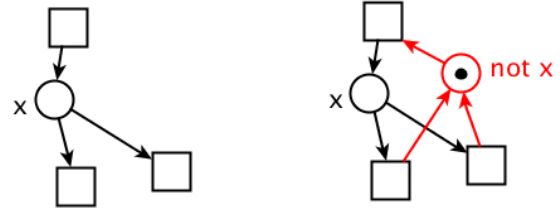
\includegraphics[width=1\linewidth]{img/contatto_complementare.png}
    \caption{Rimozione di un contatto tramite l'aggiunta dello stato complementare.}
    \label{fig:sistema_con_contatti}
\end{marginfigure}

\subsection*{Conflitto}
\begin{defn}
    Siano $\Sigma = (B, E, F, c_{\tn{start}})$ un sistema elementare,
    $e_1, e_2 \in E$ due evento e $c \in C_{\Sigma}$ una possibile
    configurazione di $\Sigma$, $e_1$ ed $e_2$ sono in \textbf{conflitto}
    in $c$ sse:
    \[
        \canFire{c}{e_1}{} \land \canFire{c}{e_2}{} \land
        \lnot \canFire{c}{\cbra{e_1, e_2}}{}
    \]
    ovvero entrambi gli eventi sono abilitati, ma il verificarsi di uno rende
    l'altro non abilitato. Di conseguenza, i due eventi non possono essere
    eseguiti in maniera concorrente. Non sapendo quale dei due eventi verrà
    effettivamente eseguito, un conflitto esprime non determinismo.

    Esistono due tipi di conflitti:
    \begin{itemize}
        \item in avanti: due eventi abilitati hanno la stessa pre-condizione.
        Il verificarsi di un evento rende falsa la pre-condizione in comune,
        disabilitando l'altro evento;
        \item all'indietro: due eventi abilitati hanno la stessa
        post-condizione. Il verificarsi di un evento rende vera la
        post-condizione in comune, disabilitando l'altro evento.
    \end{itemize}

    \begin{marginfigure}[-11cm]
        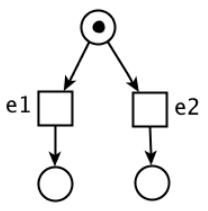
\includegraphics[width=0.75\linewidth]{img/conflitto_avanti.png}
    \caption{Conflitto in avanti.}
    \label{fig:conflitto_avanti}
    \end{marginfigure}

    \begin{marginfigure}[-3cm]
        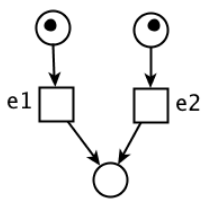
\includegraphics[width=0.75\linewidth]{img/conflitto_indietro.png}
        \caption{Conflitto all'indietro.}
        \label{fig:conflitto_indietro}
    \end{marginfigure}
\end{defn}

\subsection*{Confusione}
La confusione si presenta in un sistema con conflitti in cui la struttura non
permette di stabilire se, nel passaggio da una configurazione $c$ a una
configurazione $c'$, è stato risolto un conflitto.

\begin{figure}
    \centering
    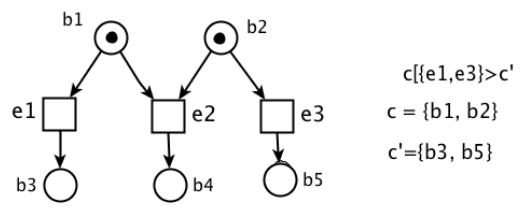
\includegraphics[width=0.5\linewidth]{img/confusione.png}
    \label{fig:confusione}
\end{figure}
In questo sistema non è possibile stabilire se, passando da $c$ a $c'$, sia
stato risolto un conflitto tra $e_1$ ed $e_2$ o tra $e_2$ ed $e_3$.

Un altro esempio di confusione si verifica nella mutua esclusione.

\subsection*{Sequenza}
Siano $\Sigma = (B, E, F, c_{\tn{start}})$ un sistema elementare,
$e_1, e_2 \in E$ due eventi e $c \in C_{\Sigma}$ una possibile configurazione
di $\Sigma$, $e_1$ ed $e_2$ sono in \textbf{sequenza} in $c$ sse:
\[
    \canFire{c}{e_1}{} \land \lnot \canFire{c}{e_2}{} \land
    \canFire{\canFire{c}{e_1}{c'}}{e_2}
\]
ovvero $e_2$ può essere eseguito sse prima viene eseguito $e_1$.
C'è quindi una dipendenza causale tra gli eventi $e_1$ ed $e_2$.

\begin{figure}
    \centering
    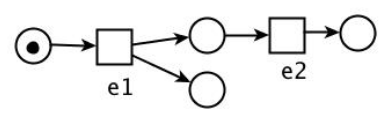
\includegraphics[width=0.5\linewidth]{img/sequenza.png}
    \caption{Due eventi in sequenza.}
    \label{fig:eventi_sequenza}
\end{figure}

\subsection*{Concorrenza}
Siano $\Sigma = (B, E, F, c_{\tn{start}})$ un sistema elementare,
$e_1, e_2 \in E$ due eventi e $c \in C_{\Sigma}$ una possibile configurazione
di $\Sigma$, $e_1$ ed $e_2$ sono \textbf{concorrenti} in $c$ sse:
\[
    \canFire{c}{\cbra{e_1, e_2}}{}
\]
ovvero $\cbra{e_1, e_2}$ è un passo abilitato. Questo significa che i due
eventi $e_1$ ed $e_2$ sono indipendenti ed entrambi abilitati in $c$.

\begin{figure}
    \centering
    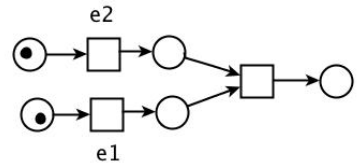
\includegraphics[width=0.5\linewidth]{img/eventi_concorrenti.png}
    \caption{Due eventi concorrenti.}
    \label{fig:eventi_concorrenti}
\end{figure}

\section{Processi non sequenziali e processi ramificati}
Prima di poter spiegare cosa sono i processi non sequenziali e i processi
ramificati, è necessario introdurre alcune nozioni.

\subsection*{Relazioni sugli elementi di una rete}
\begin{defn}
    La relazione d'ordine parziale largo \footnote{Una relazione d'ordine largo
    è una relazione riflessiva, antisimmetrica e transitiva.}
    $\le \, \subseteq (B \cup E) \times (B \cup E)$ specifica se un elemento
    è causa di un altro elemento, ed è definita come:
    \[
        \forall x, y \in B \cup E, \quad (x, y) \in \, \le \quad
        \tn{ sse } \quad x F^*y
    \]
    ovvero è possibile raggiungere $y$ a partire da $x$ usando un numero
    limitato di transizioni. Se $(x,y) \in \, \le$, allora $x$ causa $y$.
    Si può notare che, in questa relazione, un elemento $x$ causa sè stesso.
\end{defn}

\begin{defn}
    La relazione d'ordine parziale stretto \footnote{Una relazione d'ordine
    stretto è una relazione irriflessiva, asimmetrica e transitiva.}
    $< \, \subseteq (B \cup E) \times (B \cup E)$ specifica se un elemento
    è causa di un altro elemento diverso da sè stesso, ed è definita come:
    \[
        \forall x, y \in B \cup E, \quad (x, y) \in \, < \quad \tn{ sse } \quad
        x F^*y \land x \neq y
    \]
\end{defn}

\begin{rem}
    $<$ è facilmente ottenibile da $\le$ rimuovendo tutte le coppie della forma
    $(x,x), \forall x \in B \cup E$.
\end{rem}

\begin{defn}
    Sia $N$ una rete di Petri, la \textbf{relazione di conflitto}
    $\# \subseteq P \cup T$ specifica quali coppie di elementi della rete $N$
    sono causalmente dipendenti da un conflitto in avanti, ed è definita come:
    \[
        x \# y \quad \tn{ sse } \quad \exists e_1, e_2 \in E,
        (e_1 \neq e_2 \land e_1 \le x \land e_2 \le y) :
        \preCond{e_1} \cap \preCond{e_2} \neq \emptyset
    \]
\end{defn}

\begin{rem}
    La relazione di conflitto $\#$ è simmetrica ma non transitiva.
\end{rem}

\begin{defn}
    La relazione $\tn{li} \subseteq (B \cup E) \times (B \cup E)$ specifica
    quali elementi della rete sono causalmente dipendenti, ed è definita come:
    \[
        \forall x, y \in B \cup E, \quad (x, y) \in \tn{ li} \quad
        \tn{ sse } \quad (x,y) \in \, \le \lor \, (y,x) \in \, \le
    \]
\end{defn}

\begin{defn}
    La relazione $\tn{co} \subseteq (B \cup E) \times (B \cup E)$ specifica
    quali elementi della rete sono causalmente indipendenti, ed è definita come:
    \[
        \forall x, y \in B \cup E, \quad (x, y) \in \tn{ co} \quad \tn{ sse } \quad
        (x,y) \notin \, < \land \, (y,x) \notin \, < \land \, (x,y) \notin \#
    \]
\end{defn}

\begin{rem}
    \begin{align*}
        (x,y) \in \tn{ li } &\longleftrightarrow (y,x) \in \tn{ li}\\
        (x,y) \in \tn{ co } &\longleftrightarrow (y,x) \in \tn{ co}
    \end{align*}
\end{rem}
\begin{rem}
    $\tn{li}$ e $\tn{co}$ sono relazioni riflessive, simmetriche ma non
    transitive.
\end{rem}

\subsection*{Tagli e linee}
\begin{defn}
    Un \textbf{coset} $C \subseteq P \cup T$ è un insieme di elementi
    della rete di Petri tale che:
    \[
        \forall x, y \in C, x \tn{ co } y
    \]
    ovvero gli elementi di un coset sono tutti causalmente indipendenti tra
    loro.
\end{defn}

\begin{rem}
    In un coset, la relazione $\tn{co}$ è transitiva.
\end{rem}

\begin{defn}
    Un \textbf{taglio} $C \subseteq P \cup T$ è un coset massimale, ovvero:
    \[
        C \tn{ è un coset } \, \land \, \forall x \in (B \cup E) \setminus C, \,
        \exists c \in C : x \tn{ li } c
    \]
    ovvero ogni altro elemento che non appartiene a $C$ è causalmente
    dipendente da almeno un elemento di $C$, o viceversa.
\end{defn}

\begin{defn}
    Un taglio $C$ è un \textbf{P-taglio} sse $C \subseteq P$, ovvero è formato
    da soli stati locali.
\end{defn}

\begin{rem}
    Un P-taglio corrisponde a uno dei possibili casi raggiungibili della rete.
    Di conseguenza, tutti i possibili P-tagli definiscono tutti i possibili
    casi raggiungibili della rete.
\end{rem}

\begin{defn}
    Un taglio $C$ è un \textbf{T-taglio} sse $C \subseteq T$, ovvero è formato
    da soli eventi.
\end{defn}

\begin{rem}
    Tutti gli eventi all'interno di un T-taglio possono essere eseguiti in
    maniera concorrente. Essendo un T-taglio l'insieme di cardinalità massima
    $n$ che contiene solo eventi indipendenti tra loro, il sistema necessita
    di $n$ processori per l'esecuzione in minor tempo possibile degli $n$
    eventi.\\
    Il numero di processori per una rete (da cui si deriva la rete di
    occorrenze), è pari alla cardinalità massima tra le cardinalità degli
    T-tagli di tutti i processi non sequenziale che è possibile definire.
\end{rem}

\begin{defn}
    Un \textbf{liset} $L \subseteq P \cup T$ è un insieme di elementi della
    rete di Petri tale che:
    \[
        \forall x, y \in L, x \tn{ li } y
    \]
    ovvero gli elementi di un liset sono tutti causalmente dipendenti tra loro.
\end{defn}

\begin{rem}
    In un liset, la relazione $\tn{li}$ è transitiva.
\end{rem}

\begin{defn}
    Una \textbf{linea} $L \subseteq P \cup T$ è un liset massimale, ovvero:
    \[
        L \tn{ è un coset } \, \land \, \forall x \in (B \cup E) \setminus L, \,
        \exists l \in L : x \tn{ co } l
    \]
    ovvero ogni altro elemento che non appartiene a $L$ è causalmente
    indipendente da almeno un elemento di $C$, o viceversa.
\end{defn}

\subsection*{Processo ramificato}
\begin{defn}
    Una rete di Petri è una \textbf{rete di occorrenze} sse:
    \begin{itemize}
        \item $\forall p \in P, |\preCond{p}| = 1$, ovvero non sono
        accettati conflitti all'indietro. Sono invece accettati
        i conflitti in avanti.
        \item $\forall x, y \in P \cup T, (x,y) \in F^+ \rightarrow
        (y,x) \notin F^+$, ovvero non sono presenti cicli.
        \item $\forall e \in T$, l'insieme $\cbra{x \in P \cup T : x F^*e}$,
        ovvero il passato di ogni evento, ha cardinalità finita.
        \item la relazione di conflitto $\#$ è irriflessiva \footnote{E di
        conseguenza antisimmetrica.}, ovvero un unico elemento non dipende
        causalmente da due eventi in conflitto in avanti.
    \end{itemize}
\end{defn}

Su una rete di occorrenze è possibile definire le funzioni
\begin{align*}
    \tn{past}: P \cup T &\rightarrow \mathcal{P}(P \cup T)\\
    \tn{future}: P \cup T &\rightarrow \mathcal{P}(P \cup T)
\end{align*}

$\tn{past}$ restituisce tutti gli elementi della rete che causano $x$, mentre
$\tn{future}$ restituisce tutti gli elementi che sono causati da $x$.\\
Per definizione di rete di occorrenze, $\tn{past}(x)$ è sicuramente un insieme
di cardinalità finita, mentre $\tn{past}(x)$ può avere cardinalità infinita
numerabile.

\begin{rem}
    Tutti gli elementi della rete che non appartengono nè a $\tn{past}(x)$ nè
    a $\tn{future}(x)$ possono essere eseguiti in maniera concorrente rispetto
    a $x$.
\end{rem}

\begin{defn}
    Un \textbf{processo ramificato} di una rete di Petri $N_1 = (P_1, T_1, F_1, c_1)$
    senza contatti e finita (e quindi $k$-densa), è una coppia
    $(N_2, \phi), N_2 = (P_2, T_2, F_2, c_2)$ tale che:
    \begin{itemize}
        \item $N_2$ è una rete di occorrenze;
        \item $\phi: P_2 \cup T_2 \rightarrow P_1 \cup T_1$ è una funzione
        tale che:
        \begin{itemize}
            \item $\phi(P_2) \subseteq P_1 \land \phi(T_2) \subseteq T_1$
            \item $\forall e_1, e_2 \in T_2, \, (\preCond{e_1} = \preCond{e_2}
            \land \phi(e_1) = \phi(e_2)) \implies e_1 = e_2$
            \item FINIRE DEFINIZIONE
        \end{itemize}
    \end{itemize}
\end{defn}

\begin{rem}
    Un processo ramificato contiene una o più run della rete di Petri da cui
    è stato costruito.
\end{rem}

\subsection*{Processo non sequenziale}
Una rete causale è un tipo particolare di rete di occorrenze, che non presenta
alcun conflitto.\\
Una \textbf{rete causale} è una rete di Petri tale che
\footnote[][-1cm]{L'ulteriore condizione presente nelle reti di occorrenza,
ovvero che la relazione di conflitto sia irriflessiva, collassa nella prima
condizione per le reti clausali: non avendo alcun conflitto, per la rete
clausale vale $\# = \emptyset$.}:
\begin{itemize}
    \item $\forall b \in B, \lvert \preCond{b} \rvert \le 1 \land \lvert \postCond{b} \rvert \le 1$,
    ovvero non sono presenti conflitti \footnote[][1cm]{In un conflitto in
    avanti, lo stato pre-condizione ha due post-eventi. In un conflitto
    all'indietro, lo stato post-condizione ha due pre-eventi. Di conseguenza,
    imporre un numero di pre-eventi e post-eventi minore o uguale a uno implica
    l'assenza di conflitti.};
    \item $\forall x, y \in B \cup E, \quad (x, y) \in F^+ \rightarrow (y, x) \notin F^+$,
    ovvero non sono presenti cicli;
    \item $\forall e \in E$, la cardinalità dell'insieme $\cbra{x \in B \cup E | x \, F^* e}$
    è finita, ovvero i predecessori di un qualsiasi evento sono in numero
    finito.
\end{itemize}

\begin{rem}
    Una rete causale ammette elementi isolati, ovvero elementi senza archi
    in ingresso e archi in uscita.
\end{rem}

Una rete causale rappresenta una sola delle possibili esecuzioni del sistema
concorrente, ovvero un suo processo non sequenziale.
La coppia $(N, \phi)$ che definisce un processo non sequenziale
è quindi il processo non sequenziale costruito dalla rete $N$ usando la
funzione $\phi$. Diversi processi non sequenziali per la stessa rete
definiranno la funzione $\phi$ in maniera diversa ($\phi$ deve comunque
rispettare tutte le caratteristiche che deve avere la funzione che permette
di definire un processo non sequenziale).

\begin{defn}
    Un \textbf{processo non sequenziale} di una rete di Petri $N_1$
    senza contatti e finita (e quindi $k$-densa) è una coppia $(N_2, \phi)$
    tale che:
    \begin{itemize}
        \item $N_2$ è una rete causale;
        \item $\phi: B \cup E \rightarrow S \cup T$ è una funzione tale che
        FINIRE DEFINIZIONE
    \end{itemize}
\end{defn}

\begin{defn}
    Una rete è \textbf{\textit{k}-densa} se ogni linea si interseca una singola
    volta con ogni altro taglio e, viceversa, ogni taglio si interseca una
    singola volta con ogni altra linea.
\end{defn}

Un taglio e una linea si intersecano esattamente in un punto perchè se si
incontrassero in più punti, allora tutti i punti di intersezione
rappresenterebbero elementi che sono contemporaneamente casualmente
dipendenti (li) e casualmente indipendenti (co), violando quindi i tagli
e le linee definite.

\begin{rem}
    Una rete finita è sicuramente $k$-densa.
\end{rem}

\subsection*{Prefisso e unfolding}
\begin{defn}
    Sia $\Sigma = (S, T , F , c_in)$ un sistema elementare finito e senza contatti
    e siano $\Pi_1 = (N_1, \phi_1)$, $\Pi_2 = (N_2, \phi_2)$ due suoi processi
    ramificati.
    $\Pi_1$ è un prefisso di $\Pi_2$ sse:
    \begin{itemize}
        \item $N_1$ è una sottorete di $N_2$
        \item $\phi_2|N_1 = \phi_1$, ovvero $\phi_2$ ”ristretto” a $N_1$ è
        uguale a $\phi_1$.
    \end{itemize}
\end{defn}

\begin{defn}
    L'\textbf{unfolding} di una rete elementare $\Sigma$ è il processo ramificato
    massimale, ovvero il processo ramificato che include tutte le possibili
    run di $\Sigma$.
\end{defn}

\begin{rem}
    Ogni processo ramificato (compresi i processi non sequenziali, in quanto
    sono casi particolari di processi ramificati con una singola run) è un
    prefisso dell'unfolding.
\end{rem}

è possibile anche cercare di individuare un prefisso finito dell'unfolding
che permetta di derivare tutte le possibili informazioni riguardo il comportamento
del sistema elementare. Questo prefisso prende il nome di prefisso completo.


\section{Estensioni}
AGGIUNGERE RETI COLORATE, DOVE TOKEN HANNO COLORE DIVERSO.
Fino ad ora sono state considerate solo reti elementari, ovvero reti di Petri
che tollerano al massimo un token per stato e che prevedono che ogni evento
sottragga un token da ogni precondizione, e aggiunga un token a ogni
precondizione.

è possibile però anche definire reti di Petri che tollerano più token
per ogni stato (ogni stato ha una certa capacità massima) e ogni evento
può richiedere che in una sua precondizione siano presenti più di un token.
Quando l'evento scatta verranno rimossi più token da una precondizione.
Stesso ragionamento può essere applicato alle post-condizioni, in cui l'evento
aggiunge più di un token.
In entrambi casi, il fatto che vengano usati più token viene specificato mettendo
un numerino vicino all'arco che collega l'evento alla pre-condizione o alla
post-condizione.

Queste reti di Petri più ad alto livello prendono il nome di reti Posti e Transizioni.
Reti elementari e reti Posti e Transizioni hanno la stessa capacità espressiva:
le reti Posti e Transizioni permettono semplicemente di definire una rete
più compatta, e quindi più facile da rappresentare.

Su una rete Posti e Transizioni in cui ogni stato ha capacità infinita
e non sono presenti cappi, allora è possibile definire una matrice di incidenza:
le righe corrispondono agli stati, mentre le colonne alle transizioni;
il peso degli archi sarà semplicemente il numero di token rimossi, se l'arco
va da precondizione a evento, o token aggiunti, se l'arco va da evento a
post-condizione.

La matrice di incidenza può essere usata per simulare le transizioni.
Sia infatti $M_i$ la configurazione corrente della rete, rappresentata come
una colonna "in più" della matrice in cui si associa a ogni stato il numero
di token, allora si può trovare la prossima configurazione della rete
allo scattare dell'evento $t$ semplicemente sommando la colonna associata
alla configurazione di partenza e la colonna associata a $t$.
La nuova colonna ottenuta è la nuova configurazione.

Si può affermare quindi che una configurazione $M_1$ è raggiungibile
da $M_0$ allo scattare di $t$, ovvero $M_0[t>M_1$ sse $M_0 + t = M_1$.
Questa equazione prende il nome di equazione di stato.

Sulle reti Posti e Transizioni con capacità infinita per ogni stato
possono essere definite delle proprietà:
\begin{itemize}
    \item la rete è limitata (bounded)  sse
    \item safe
    \item terminante sse non ammette sequenze infinite
    \item deadlock-free
    \item live sse
    \item reversibile/ciclico
    \item FINIRE
\end{itemize}

Queste proprietà possono essere verificate algoritmicamente (non visto durante
il corso).

\chapter{Model checking}
\section{Introduzione}
Quando si sviluppano sistemi software complessi, è importante che il sistema
rispetti tutti i requisiti definiti in fase di progettazione.
Questi requisiti, molto spesso, sono espressi in linguaggio naturale, e vengono
poi affiancati da rappresentazioni grafiche, come diagrammi UML.
Definire però correttamente tutti i requisiti di un sistema software
complesso risulta molto
: oltre che garantire la presenza di tutti i requisiti richiesti, bisogna
controllare che essi non siano ambigui e non si contraddicano.
Verificare queste caratteristiche algoritmicamente risulta però complicato:
il linguaggio naturale, usato appunto per descrivere i requisiti, risulta
molto complesso da analizzare e, allo stato attuale impreciso.
Per questo, si è deciso di trattare i requisiti e la loro verifica in
maniera più formale, ed è stato introdotto il model checking.
Il model checking è un metodo per verificare algoritmicamente la correttezza di
sistemi formali. In particolare, il model checking prevede di rappresentare
il sistema considerato come un modello formale \footnote{Con
modello del sistema si intende la sua implementazione.},
solitamente un sistema a transizioni etichettato, e di descrivere la specifica
\footnote{La specifica è una proprietà che deve essere rispettata dal sistema.},
ovvero i requisiti, usando un linguaggio preciso e non ambiguo, solitamente
la logica temporale, e utilizza algoritmi ben definiti per stabilire
se la specifica, o altre proprietà desiderate, è verificata nel modello
che rappresenta il sistema. Se una certa proprietà non è rispettata nel modello,
inoltre, il model checking prevede di fornire una dimostrazione, ovvero una
traccia di esecuzione che funge da controesempio alla proprietà considerata.

Una logica temporale è un'estensione della logica proposizionale classica,
in cui la struttura di interpretazione è una successione di istanti di tempo
distinti.
Non esiste un'unica logica temporale, ma ne esistono molteplici, tutte
sotto del $\mu$-calcolo, una logica modale.
Qui verranno analizzate la Linear Temporal Logic e la Computational Tree
Logic.


\section{Modelli di Kripke}
Il model checking viene effettuato su modelli detti modelli di Kripke,
che altro non sono che sistema a transizioni non etichettati in cui
a ogni stato è associato un sottoinsieme di proprietà valide in quello stato.
Vengono quindi introdotte alcune nozioni necessarie per trattare i modelli di
Kripke.

\begin{defn}
    Un \textbf{sistema di transizioni} è una coppia $(Q, T)$ dove:
    \begin{itemize}
        \item $Q$ è un insieme di stati \footnote[][1cm]{L'insieme di stati
        può essere infinito, anche non numerabile. In queste note, a meno che
        venga esplicitato, si tratteranno sistemi di transizioni finiti,
        ovvero con un insieme di stati finito.}.
        \item $T \subseteq Q \times Q$ è la relazione di transizione, ovvero
        quella relazione che stabilisce i collegamenti tra stati del sistema.
    \end{itemize}
\end{defn}

\begin{rem}
    In un sistema di transizioni non etichettato, per ogni coppia di nodi $u$
    e $v$ può essere presente al massimo un arco $(u, v)$ che li collega.
\end{rem}

\begin{defn}
    Un \textbf{cammino} è una sequenza finita di stati
    $q_0 q_1 \ldots q_k, q_i \in Q$.
\end{defn}

\begin{defn}
    Un \textbf{cammino massimale} è un cammino che non può essere esteso.
\end{defn}

\begin{defn}
    Il \textbf{modello di Kripke} è una tripla:
    \[
        (Q, T, I)
    \]
    dove:
    \begin{itemize}
        \item $(Q, T)$ è un sistema di transizioni che rappresenta il sistema
        concorrente;
        \item $I: Q \rightarrow \mathcal{P}(AP)$ è una funzione che associa a
        ogni stato un sottoinsieme di proposizioni atomiche vere in quello
        stato. $I$ viene detta \textbf{funzione di interpretazione}.\\
        $I(q)$ indica il sottoinsieme di proposizioni atomiche vere in $q$.
    \end{itemize}
\end{defn}

A ogni stato $q$ è associato un insieme di cammini massimali per quello stato.\\
Una WFF è vera in uno stato $q$ sse è vera per tutti i cammini massimali che
partono da $q$. Se una WFF $p$ è vera in un certo cammino $\pi$, allora si
scrive $\pi \vDash p$.

Un sistema concorrente rappresentato tramite un modello di Kripke soddisfa una
specifica, ovvero una WFF della LTL, sse la specifica è vera per tutti i
cammini massimali che partono dallo stato iniziale.

Due modelli di Kripke $M_1$ e $M_2$, con stati iniziali rispettivamente
$q_0$ e $s_0$, sono equivalenti rispetto a una logica $L$ sse $\forall \alpha \in L$,
ovvero per tutte le formule della logica,
\[
    M_1, q_0 \vDash \alpha \longleftrightarrow M_2, s_0 \vDash \alpha
\]
ovvero se una formula logica vale nello stato iniziale di un modello, allora
deve valere anche nello stato iniziale dell'altro modello.

\section{Logiche temporali}
\subsection{Linear Temporal Logic}
La Linear Temporal Logic è una logica modale temporale in cui le modalità
fanno riferimento al tempo. In particolare, LTL permette di esprimere
proprietà su un tempo discreto, organizzato linearmente, infinito
e orientato al futuro.

La LTL presenta però dei limiti: essa non può, infatti, esprimere
proprietà riguardanti insiemi di cammini, ovvero non può richiedere
che una certa proprietà sia rispettata da tutti i cammini o da almeno un
cammino.
Un esempio di proprietà che non può essere espressa in LTL è la reset property,
ovvero che da ogni stato di qualsiasi cammino sia possibile raggiungere
uno stato in cui vale una certa proprietà.

\subsection*{Sintassi e semantica LTL}
Sia $AP$ l'insieme delle proposizioni atomiche, $p \in AP$ una proposizione
atomica, e $\alpha, \beta$ due WFF della LTL.
L'insieme $WFF_{\tn{LTL}}$ delle formule ben formate della LTL è definito come:
\begin{itemize}
    \item $p \in WFF_{\tn{LTL}}$,
    \item $\tn{true}, \tn{false} \in WFF_{\tn{LTL}}$
    \item $\alpha \lor \beta \in WFF_{\tn{LTL}}$ e $\lnot \alpha \in WFF_{\tn{LTL}}$
    \item $\nextOp \alpha \in WFF_{\tn{LTL}}$
    \item $\finallyOp \alpha \in WFF_{\tn{LTL}}$
    \item $\globallyOp \alpha \in WFF_{\tn{LTL}}$
    \item $\untilOp \alpha \in WFF_{\tn{LTL}}$
\end{itemize}

Siano $\pi = q_0 q_1 \ldots, q_i \in Q$ un cammino definito sul modello di
Kripke, e $\alpha, \beta \in WFF_{\tn{LTL}}$.
\begin{itemize}
    \item $\pi \vDash p \longleftrightarrow p \in I(q_0)$, ovvero $p$ vale
    nello stato iniziale $q_0$ di $\pi$.
    \item $\pi \vDash \lnot \alpha \longleftrightarrow \pi \nvDash \alpha$
    \item $\pi \vDash \alpha \lor \beta \longleftrightarrow \pi \vDash \alpha \lor \pi \vDash \beta$
    \item $\pi \vDash \nextOp \beta \longleftrightarrow \pi^{(1)} \vDash \beta$,
    ovvero $\beta$ vale nello stato successivo $\pi^{(1)}$.
    \marginnote{$\nextOp = \tn{neXt}$\\
    $\finallyOp = \tn{Finally}$\\
    $\globallyOp = \tn{Globally}$\\
    $\untilOp = \tn{Until}$}
    \item $\pi \vDash \finallyOp \beta \longleftrightarrow
    \exists i \in \mathbb{N} : \pi^{(i)} \vDash \beta$,
    ovvero $\beta$ vale in almeno uno stato del cammino $\pi$.
    \item $\pi \vDash \globallyOp \beta \longleftrightarrow
    \forall i \in \mathbb{N} : \pi^{(i)} \vDash \beta$,
    ovvero $\beta$ vale in ogni stato del cammino $\pi$.
    \item $\pi \vDash \alpha \untilOp \beta \longleftrightarrow
    (\pi \vDash \finallyOp \beta) \land
    (\forall h \in \mathbb{N}, h < i : \pi^{(i)} \vDash \alpha)$,
    ovvero $\beta$ è vera in almeno uno stato $q_i$ del cammino e in ogni stato
    precedente a $q_i$ vale $\alpha$.
    \item $\pi \vDash \alpha \weakOp \beta \longleftrightarrow
    \pi \vDash \globallyOp \alpha \lor (\alpha \lor \beta)$, ovvero
    si comporta come l'operatore $\untilOp$ ma non è detto che $\beta$ prima
    o poi diventi vera.
    \item $\pi \vDash \alpha \releaseOp \beta \longleftrightarrow
    \pi \vDash \beta \weakOp (\alpha \land \beta)$, ovvero vale $\beta$
    fino a quando non valgono contemporaneamente $\alpha$ e $\beta$ nello
    stesso stato. Non è però detto che $(\alpha \land \beta)$ prima o
    poi sia vero (c'è l'operatore weak), e quindi in questo caso
    sarà sempre vero $\beta$.
\end{itemize}

In realtà, gli operatori LTL visti fin'ora non formano un insieme minimale
di operatori: alcuni di essi, infatti, possono essere derivati dagli altri.
Di conseguenza, è possibile definire un insieme minimale di operatori.
LTL ammette più insiemi minimali di operatori; uno di questi è
$\cbra{\nextOp, \untilOp}$.

\subsection*{Esempi di formule LTL}
\begin{itemize}
    \item $\finallyOp \globallyOp \alpha$: $\alpha$ è invariante da un certo
    istante in poi.
    \item $\globallyOp \finallyOp \alpha$: $\alpha$ è vera in un numero
    infinito di stati.
    \item $\globallyOp \lnot (c_1 \land c_2)$: mutua esclusione. $c_1$ e
    $c_2$ sono le sezioni critiche dei due processi che interagiscono.
    \item $\globallyOp (\text{req} \rightarrow \nextOp \finallyOp \text{ack})$:
    ogni richiesta viene sempre prima o poi gestita.
    \item $\globallyOp (\text{req} \rightarrow (\text{req} \untilOp \text{ack}))$:
    fino a quando la richiesta viene gestita, la richiesta rimane pending.
\end{itemize}

\subsection*{Algoritmo di model checking per LTL}
L'algoritmo di model checking per LTL prevede di costruire un automa di
B\"uchi per la formula LTL e costruire un automa a stati finiti etichettato
a partire dal modello di Kripke, per poi verificare se l'intersezione
tra i due automi, ovvero il loro prodotto sincrono, riconosce il linguaggio
vuoto. Solo in questo caso, infatti, la formula LTL risulta verificata
sul modello di Kripke preso in considerazione.

\begin{defn}
    Un \textbf{automa di Buchi} è una quintupla $(Q, \Sigma, \delta, q_0, F)$
    dove:
    \begin{itemize}
        \item $Q$ è un insieme finito di stati;
        \item $\Sigma$ è l'alfabeto di input;
        \item $\delta : Q \times \Sigma \rightarrow Q$ è la funzione di transizione;
        \item $q_0$ è lo stato iniziale.;
        \item $F$ è un sottoinsieme di stati finali.
    \end{itemize}
    A differenza di un classico automa a stati finiti, però, la condizione di
    accettazione di un automa di B\"uchi è che la sequenza (infinita)
    di transizioni compiute sulla parola in ingresso attraversi almeno uno
    stato finale per un numero infinito di volte.
    Di conseguenza, l'automa di B\"uchi può accettare anche stringhe infinite
    sull'alfabeto finito $\Sigma$.
\end{defn}

Siano $M = (Q, T, I)$ il modello di Kripke considerato, $q_0$ il suo stato
iniziale, e $\alpha$ la formula LTL che si vuole verificare su $M$.
L'algoritmo che permette di stabilire se $\alpha$ è valida nello stato iniziale
di $M$, ovvero $q_0$, è il seguente:
\begin{enumerate}
    \item Costruisco l'automa di B\"uchi $B_{\lnot \alpha}$ che riconosce
    tutte le stringhe in cui non vale la formula $\alpha$;
    \item Trasformo l'automa di B\"uchi $M$ in un automa a stati finiti $S$,
    i cui archi sono etichettati con elementi di $2^{AP}$, ovvero i sottoinsiemi
    di proposizioni atomiche che la funzione di interpretazione $I$ assegna
    agli stati del modello di Kripke.
    \item Calcolo il prodotto sincrono $A_{\lnot \alpha} S$ tra l'automa
    $A_{\lnot \alpha}$ e l'automa $S$.
    \item Se il linguaggio riconosciuto dall'automa generato dal prodotto sincrono
    tra i due automi è l'insieme vuoto, allora in $q_0$ vale $\alpha$, ovvero
    $M, q_0 \vDash \alpha$. Di conseguenza, la formula $\alpha$ è verificata
    nel modello $M$.
\end{enumerate}


La complessità dell'algoritmo di model checking per formule LTL
risulta essere:
\[
    T(M, \alpha) = O(|M| \cdot 2^{|\alpha|})
\]
ed è quindi esponenziale.
Le formule che solitamente si vogliono verificare, però, sono molto spesso
di dimensioni ridotte, e la crescita esponenziale è contenuta.
Al contrario, i modelli di Kripke presi in analisi sono solitamente di grandi
dimensioni e sono, di fatto, il fattore più determinante nella crescita della
funzione di complessità.

\subsection{Computational Tree Logic}
La Computational Tree Logic è una logica temporale in cui il tempo è discreto
e organizzato in una struttura ad albero, in cui il futuro da intraprendere
ad un determinato punto di branch non è predeterminato.

La CTL permette di esprimere un sottoinsieme stretto di formule della LTL
e, quindi, non coincide con LTL.
Un esempio di proprietà esprimile in CTL ma non LTL è la reset property, ovvero
$A \globallyOp E \finallyOp p$.

Sintassi:
\begin{itemize}
    \item Proposizione atomiche sono formule valide
    \item la negazione di formule ben formate è una formula ben formata
    \item stessa cosa per implicazione, congiunzione, disgiunzione.
    \item $AX \alpha, EX \alpha$ sono FBF
    \item $AF \alpha, EF \alpha$ sono FBF
    \item $AG \alpha, EG \alpha$ sono FBF
    \item $A(\alpha \untilOp \beta), E(\alpha \untilOp \beta)$ sono FBF
\end{itemize}

A ed E sono quantificatori sui cammini: A indica per ogni cammino, mentre
E indica esiste un cammino tale che.

\subsection*{Nozioni utili per definire un algoritmo di model cheching per CTL}
Un insieme parzialmente ordinato $(A, \le)$, detto anche poset, è una struttura
algebrica formata da un insieme di elementi $A$ e una relazione d'ordine parziale
$\le$ definita su $A$.
Una relazione binaria è una relazione d'ordine parziale sse è riflessiva,
antisimmetrica e transitiva.
In una relazione d'ordine parziale $R$, non è garantito che
$\forall x, y \in A, (x,y) \in R \lor (y,x) \in R$, ovvero non è garantito
che tutti gli elementi siano confrontabili.

Sia $B \subseteq A$ un sottoinsieme di elementi di $A$:
\begin{itemize}
    \item $x \in A$ è un maggiorante di $B$ sse $\forall y \in B, y \le x$.
    \item $x \in A$ è un minorante di $B$ sse $\forall y \in B, x \le y$.
\end{itemize}
Non è sempre garantito che qualsiasi sottoinsieme $B$ ammetta maggiorante
e minorante.
Se $B$ ammette almeno un maggiorante, allora si dice che $B$ è limitato
superiormente.
Se $B$ ammette almeno un minorante, allora si dice che $B$ è limitato
inferiormente.

$x \in B$ è il minimo di $B$ sse $\forall y \in B, x \le y$.
$x \in B$ è il massimo di $B$ sse $\forall y \in B, y \le x$.

L'estremo inferiore di $B$ è il massimo dei minoranti.
L'estremo superiore di $B$ è il minimo dei maggioranti.

\begin{defn}
    Un \textbf{reticolo} (detto anche lattice) è un insieme parzialmente ordinato $(L, \le)$ in cui
    qualsiasi coppia di elementi ammette un estremo superiore e un estremo
    inferiore, ovvero:
    \[
        \forall x, y \in L, \exists x \bigvee y \land \exists x \bigwedge y
    \]
\end{defn}

\begin{defn}
    Un reticolo è un \textbf{reticolo completo} sse
    \[
        \forall B \subseteq L, \exists \bigvee B \land \exists \bigwedge B
    \]
\end{defn}

\begin{defn}
    Dati due poset $(L_1, \le_1)$ e $(L_2, \le_2)$.
    Una funzione $f: L_1 \rightarrow L_2$ si dice \textbf{monotona} sse
    \[
        \forall x,y \in L_1, \quad x \le_1 y \rightarrow f(x) \le_2 f(y)
    \]
\end{defn}

\begin{defn}
    Data una funzione generica $f: X \rightarrow X$.
    Un elemento $x \in X$ è un punto fisso per la funzione $f$ sse $f(x) = x$.
\end{defn}

\begin{exmp}
    I punti fissi della funzione $f: \mathbb{R} \rightarrow \mathbb{R}, f(x) = x^2$
    sono 0 e 1.\\
    La funzione $f: \mathbb{R}^+ \rightarrow \mathbb{R}, f(x) = \log_2(x)$
    non ha alcun punto fisso.
\end{exmp}

\begin{thm}[Teorema di Knaster-Tarski]
    Sia $(L, \le)$ un reticolo completo, e $f: L \rightarrow L$ una funzione
    monotona non descrescente. Allora l'insieme dei punti fissi di $f$ è un reticolo completo
    e, di conseguenza, $f$ ammette un minimo punto fisso e un massimo punto
    fisso.

    \begin{proof}
        La dimostrazione qui effettuata considera solo un caso particolare,
        ovvero quello in cui il reticolo completo è $(2^A, \subseteq)$,
        e non si può quindi considerare completa.

        Si può innanzitutto costruire un insieme $Z$ di \textit{punti prefissi}.
        \[
            Z = \cbra{T \subseteq A \, | \, f(T) \subseteq T}
        \]
        ovvero l'insieme contenente tutti gli elementi del reticolo completo
        che sono sottoinsiemi della loro stessa immagine.
        Sicuramente $Z \neq \emptyset$, in quanto vale sicuramente
        $f(A) \subseteq A$, e quindi $A \in Z$.

        La dimostrazione è strutturata in 3 punti:
        \begin{enumerate}
            \item dimostrare che l'insieme $Z$ contiene tutti i punti
            fissi della funzione $f$.
            \item dimostrare che il minimo $m$ di $Z$ appartiene a $Z$ stesso.
            \item dimostrare che $m$ è punto fisso della funzione $f$.
        \end{enumerate}
        Dopo aver dimostrato questi tre punti, si può concludere che
        $m$ è il minimo punto fisso della funzione $f$.

        \begin{enumerate}
            \item Si può notare che, se la funzione $f$ ammette punti fissi,
            allora i punti fissi di $f$ sicuramente appartengono a $Z$.
            \item Una volta calcolato l'insieme $Z$, che altro non è che un
            insieme di elementi del reticolo, è possibile calcolare
            il suo estremo inferiore. Questa operazione è sicuramente possibile,
            in quanto $(2^A, \subseteq)$ è un reticolo completo e, di conseguenza,
            ogni sottoinsieme di $2^A$ ammette estremo inferiore ed estremo superiore.\\
            \[
                m = \bigcap Z
            \]
            Ovviamente si può affermare che $m \subseteq S, \forall S \in Z$, per
            definizione di estremo inferiore nel reticolo completo $(2^A, \subseteq)$.

            Essendo però $f$ una funzione monotona su $(2^A, \subseteq)$,
            allora vale:
            \[
                m \subseteq S \longrightarrow f(m) \subseteq f(S) \subseteq S \quad
                \forall S \in Z
            \]
            $f(m)$ è sottoinsieme di ogni elemento di $Z$, ovvero
            $f(m) \subseteq S, \forall S \in Z$, sse $f(m) \subseteq \bigcap Z$.
            Però $\bigcap Z = m$ e, di conseguenza, vale $f(m) \subseteq m$.
            Ma, per come è definito l'insieme $Z$, allora
            vale sicuramente $m \in Z$. Di conseguenza, si è dimostrato che il
            minimo di $Z$ appartiene a $Z$ stesso.
            \item Manca solo dimostrare che $m$ è effettivamente un punto fisso
            della funzione $f$. Avendo dimostrato che $f(m) \subseteq m$, dimostrare
            la relazione opposta, ovvero $m \subseteq f(m)$, permetterebbe
            di concludere che $m$ è punto fisso, in quanto di otterrebbe
            $f(m) = m$.

            Si è precedentemente dimostrato nel punto 2 che vale
            $f(m) \subseteq m$. Essendo $f$ una funzione monotona,
            applicando la funzione $f$ a entrambi i membri della disuguaglianza
            si ottiene $f(f(m)) \subseteq f(m)$.
            Ma, per come è stato definito $Z$, allora vale $f(m) \in Z$.
            L'estremo inferiore $m$ di $Z$, per definizione di estremo inferiore,
            è sicuramente sottoinsieme di ogni elemento di $Z$: si può quindi
            affermare che $m \subseteq f(m)$.

            Avendo dimostrato $f(m) \subseteq m$ e $m \subseteq f(m)$,
            allora si può concludere che $f(m) = m$. Di conseguenza,
            $m$ è un punto fisso di $f$.
        \end{enumerate}
        Avendo dimostrato che $Z$ contiene tutti i punti fissi della funzione $f$,
        il minimo $m$ di $Z$ appartiene a $Z$ stesso e $m$ è un punto fisso,
        allora si può concludere che $m$, calcolato come l'intersezione di
        tutti i sottoinsiemi di $A$ contenuti in $Z$, è il suo minimo
        punto fisso.

        Lo stesso ragionamento può essere applicato per dimostrare l'esistenza
        del massimo punto fisso: l'unica differenza sta nel fatto che
        il sottoinsieme $m$ non verrà più calcolato come estremo inferiore
        di $Z$, ma come estremo superiore.
    \end{proof}
\end{thm}

Il teorema di Knaster-Tarski afferma che una funzione monotona
crescente su un reticolo completo ammette sempre un minimo punto fisso
e un massimo punto fisso. Non specifica, però, un vero e proprio
algoritmo di calcolo per questi punti fissi.
Il metodo di calcolo viene, invece, esposto nel teorema di Kleene.

\begin{thm}[Teorema di Kleene]
    Sia $(L, \le)$ un reticolo completo, e $f$ una funzione continua
    secondo Scott, e quindi monotona.\\
    Il minimo punto fisso di $f$ è l'estremo superiore della
    catena di Kleene crescente su $f$ che parte da $\bot$:
    \[
        \bot \le f(\bot) \le f(f(\bot)) \le \ldots \le f^n(\bot) \le \ldots
    \]
    dove $\bot$ è il minimo del reticolo completo $(L, \le)$.

    Il massimo punto fisso di $f$ è l'estremo superiore della catena
    di Kleene crescente su $f$ che parte da $\top$:
    \[
        \top \le f(\top) \le f(f(\top)) \le \ldots \le f^n(\top) \le \ldots
    \]
    dove $\top$ è il massimo del reticolo completo $(L, \le)$.

    \begin{rem}
        Il minimo punto fisso è calcolato applicato iterativamente $f$
        a partire dal minimo del reticolo completo $(L, \le)$, fino
        a quando il risultato fornito dalla funzione è uguale all'ultimo
        argomento.

        Il massimo punto fisso è calcolato allo stesso modo, ma a partire
        dal massimo del reticolo completo $(L, \le)$.
    \end{rem}
\end{thm}

\subsection*{Algoritmo per model checking con CTL}
Per poter spiegare l'algoritmo di model checking per CTL, è necessario prima
capire cos'è l'estensione di una formula $\alpha$.
\begin{defn}
    Sia $M = (Q, T, I)$ un modello di Kripke e $\alpha$ una formula CTL.
    L'\textbf{estensione} di $\alpha$ è un sottoinsieme di stati del modello
    in cui vale $\alpha$.
    \[
        \llbracket \alpha \rrbracket = \cbra{q \in Q \,|\, M, q \vDash \alpha}
    \]
\end{defn}

Si consideri ora un modello di Kripke $M = (Q, T, I)$ su cui si vuole
valutare una formula CTL $\alpha$.
$(2^Q, \le)$ è un reticolo completo, dove $\le$ è una relazione di ordine
temporale.
\upperAccE possibile definire, per ogni operatore CTL, un'apposita funzione,
la quale permette di calcolare l'estensione dell'operatore CTL applicato
a una formula $\alpha$ a partire dall'estensione di $\alpha$. In particolare,
le estensioni degli operatori CTL sono minimi o massimi punti fissi
per le rispettive funzioni associate.

COMPLETARE CON TUTTE LE REGOLE

Si consideri $\alpha \equiv A \finallyOp \beta$.
Si può definire la funzione $f_{\alpha} : 2^Q \longrightarrow 2^Q$ come:
\[
    f_{\alpha}(H) = \llbracket \beta \rrbracket \cup
    \cbra{q \in Q \, | \, \forall (q, q') \in T : q' \in H}
    \quad H \subseteq Q
\]
ovvero la funzione $f_{\alpha}$ aggiunge all'estensione $\llbracket \beta \rrbracket$
tutti gli stati del modello di Kripke per cui tutti gli archi uscenti
finiscono in uno stato contenuto in $\llbracket \beta \rrbracket$.

Si può affermare che $\llbracket \alpha \rrbracket$, ovvero l'estensione
di $\alpha$, è il minimo punto fisso di $f_{\alpha}$, e può essere calcolato
secondo il teorema di Kleene.

Si consideri ora $\alpha \equiv E \globallyOp \beta$.
Si può definire la funzione $g_{\alpha} : 2^Q \longrightarrow 2^Q$ come:
\[
    g_{\alpha}(H) = \llbracket \beta \rrbracket \cap
    \cbra{q \in Q \, | \, \exists(q, q') \in T : q' \in H} \quad
    H \subseteq Q
\]
ovvero la funzione $g_{\alpha}$ aggiunge all'estensione
$\llbracket \beta \rrbracket$ tutti gli stati del modello di Kripke
per cui esiste almeno un arco uscente che finisce in uno stato contenuto
in $\llbracket \beta \rrbracket$.

Si può affermare che $\llbracket \alpha \rrbracket$, ovvero l'estensione
di $\alpha$, è il massimo punto fisso di $g_{\alpha}$, e può essere
calcolato secondo il teorema di Kleene.

La complessità dell'algoritmo di model checking per CTL è pari a:
\[
    T(M, \alpha) = O(|M| \cdot |\alpha|)
\]
SI può quindi affermare che il model checking di una formula CTL
risulta computazionalmente più efficiente del model checking di una formula
LTL.

\subsection{Confronto tra logiche temporali}
Alcune proprietà possono essere espresse sia in LTL che in CTL.
Esempi sono le invarianti:
\[
    A \globallyOp \lnot p \equiv G \lnot p
\]
Reattività:
\[
    A \globallyOp (p \rightarrow A \finallyOp  q) \equiv
    G (p \rightarrow \finallyOp q)
\]

Alcune proprietà CTL non possono essere espresse in LTL.
Un esempio è la reset property, ovvero che da ogni stato raggiungibile
in ogni cammino sia sempre possibile raggiungere uno stato in cui vale
$p$. Reset property in CTL:
\[
    A \globallyOp E \finallyOp p
\]

Un esempio di formula LTL che invece non si può esprimere in CTL è
$\finallyOp \globallyOp p$, ovvero che in ogni cammino, prima o poi
$p$ diventa sempre vera.

\section{Limiti del model checking}
Nei precedenti capitoli sono stati studiati alcuni modelli formali,
come le algebre di processo e le reti di Petri, che permettono di
rappresentare i sistemi reattivi, ovvero tutti quei sistemi
concorrenti, distribuiti e asincroni, che non obbediscono al paradigma
input-computazione-output, in quanto idealmente non hanno uno stato
di partenza e non terminano, ma continuano a offrire le loro funzionalità.

A partire da questi modelli, è possibile definire i relativi modelli di Kripke,
in modo da poter verificare alcune proprietà sul sistema e stabilirne
quindi la correttezza. Questa costruzione molto spesso, però, può portare
a un'esplosione combinatoria degli stati, aumentando notevolmente
i tempi di verifica e la quantità di memoria richiesta per rappresentarli.
Per questo motivo, usando i modelli "puri" visto fin'ora, possono essere
analizzati in un tempo ragionevole solo modelli con un numero di stati
che si aggira intorno al milione.

Nel corso degli anni, però, sono state sviluppate tecniche, come
gli algoritmi simbolici
\footnote{Gli algoritmi simbolici permettono di rappresentare lo spazio
degli stati del modello di Kripke usando delle funzioni, evitando quindi
di doverlo memorizzare esplicitamente e contenendo quindi la quantità
di memoria richiesta.},
il Bounded Model Checking
\footnote{Il Bounded Model Checking genera lo spazio degli stati fino a
una profondità prefissata, e verifica la formula solo sugli stati generati.
Il risultato di un Bounded Model Checking è quindi ternario: la formula
è verificata, la formula non è verificata, e non è possibile stabilire
se la formula è verificata.
Si può dimostrare, inoltre, che esiste una riduzione dal problema BMC a SAT:
BMC può quindi essere risolto usando algoritmi di SAT solving.}
e il model checking al volo
\footnote{Il model checking al volo prevede di tenere in memoria solo quegli
stati del modello di Kripke utili nella dimostrazione della formula temporale
considerata, evitando quindi di memorizzare tutti gli stati e riducendo
l'esplosione combinatoria.},
che permettono di memorizzare più efficacemente gli stati,
contenendo quindi l'esplosione combinatoria, e di velocizzare i tempi di verifica.
L'utilizzo di queste tecniche permette di trattare modelli di Kripke che possono
raggiungere un numero di stati elevatissimo, che si aggira intorno a $10^{120}$.

\section{Model checking e sviluppo software}
L'utilizzo del model checking nello sviluppo software si traduce principalmente
in quello che prende il nome di \textit{paradigma model based}: in questo paradigma
di programmazione, lo sviluppo è guidato da modelli formali del sistema
che si vuole implementare, su cui vengono verificate formule logiche
temporali, in modo da stabilirne la correttezza.
In particolare, questo paradigma prevede che, prima ancora di
di scrivere il codice, i requisiti vengano completamente modellati
con un modello di Kripke e controllati tramite model checking, in modo da
rilevare più errori possibili nell'implementazione e anticiparli
il più possibile nel processo di sviluppo. Solo dopo aver effettuato una
fase di model checking adeguata, allora il sistema potrà essere effettivamente
implementato tramite scrittura di codice.
Avendo però già descritto il sistema come un modello formale, molto spesso
la scrittura di codice a partire dal modello può essere effettuata da
traduttori automatici, contenendo il tempo richiesto per l'implementazione:
in questo modo, la maggior parte delle risorse può essere concentrata
sulla fase iniziale di modellazione e model checking, assicurando un'alta
qualità del software.

Un altro approccio che può essere utilizzato prende il nome di
\textit{Software Model Checking}, e consiste nel tradurre codice già scritto
in un modello di Kripke, in modo da poter verificarne alcune proprietà
tramite model checking. Questo approccio risulta più complesso, in quanto
già solo due variabili a 32 bit generano uno spazio degli stati con $2^{64}$
elementi. Sono stati comunque sviluppati tool che permettono di verificare
alcune proprietà sul codice, e in alcuni casi che accettano direttamente
in input il codice stesso, senza la necessità di convertirlo prima in un
modello di Kripke
\footnote{Esempi di software model checker sono SLAM (C),
CMBC (C++) e JavaPathFinder (Java)}.\\

\section{SPIN e NuSVM: tool per il model checking}

\section{SLAM: software model checker per il linguaggio C}

\section{Approfondimento: $\mu$-calcolo e fairness}
\subsection*{$\mu$-calcolo}
Il $\mu$-calcolo è un superset del $\text{CTL}^*$: ogni formula esprimibile
in LTL, CTL e $\text{CTL}^*$ può quindi essere riscritta in $\mu$-calcolo.

Il $\mu$-calcolo ha quindi la massima espressività, ma ha un'alta complessità
e le sue formule sono molto difficili da interpretare.

\subsection*{Sintassi $\mu$-calcolo}
Sia $AP$ l'insieme delle proposizioni atomiche, $p \in AP$ una proposizione
atomica, $A$ l'insieme finito delle azioni, e $V$ l'insieme
numerabile delle variabili.
L'insieme $WFF_{\mu}$ delle formule ben formate del $\mu$-calcolo è definito come:
\begin{itemize}
    \item $p \in WFF_{\mu}$,
    \item $\tn{true}, \tn{false} \in WFF_{\mu}$
    \item $\alpha \lor \beta \in WFF_{\mu}$ e $\lnot \alpha \in WFF_{\mu}$
    \item $[a]\phi \in WFF_{\mu}$
    \item $\ang{a}\phi \in WFF_{\mu}$
    \item $v Z . \phi \in WFF_{\mu}$
    \item $\mu Z . \phi \in WFF_{\mu}$
\end{itemize}


\subsection*{Semantica $\mu$-calcolo}
La semantica del $\mu$-calcolo è definita su modelli di Kripke attraverso
operatori di punto fisso.

\subsection*{Fairness}
Un evento è unfair se rimane sempre abilitato.
Si può quindi definire il concetto di fairness, che impedisce che
l'esecuzione della rete sia ingiusto e prediliga alcuni eventi rispetto
ad altri.

Esistono due tipi di fairness:
\begin{itemize}
    \item fairness debole: se un evento è abilitato, allora prima o poi
    diventerà disabilitato.
    \item fairness forte: se un evento è abilitato, allora prima o poi
    scatterà.
\end{itemize}


\printbibliography

\end{document}
